\section{Density matrix and entropy for complex network}
%as in paper 2023 with the special case in paper 2020
The communicability matrix defined above possesses peculiar properties that make it suitable for use as a density matrix. Moreover, the presence of the Laplacian matrix ensure that it does not only consider the topological features of the network but also the dynamics. Taking the exponential communicability matrix as a reference, we can define a density matrix as
\begin{equation}\label{density_matrix}
    \hat \rho(\beta) = \frac{1}{Z} e^{-\beta \hat L} \qquad \mathrm{with} \qquad Z(\beta) = \Tr[e^{-\beta \hat L}],
\end{equation}
where $Z$ is the partition function and it is equal to the Laplacian Estrada index of the network \eqref{EE_L}.
It is a hermitian and positive defined matrix with trace equal to unity. 
It can be seen that $e^{-\beta L}$ is the propagator for diffusion equation in a network at time $t = \beta$.

From this, we can define the network's entropy as the Von Neumann entropy
\begin{equation} \label{entropy}
    S(\hat\rho) = -\Tr[\hat \rho \ln \hat \rho].
\end{equation}

Considering \eqref{density_matrix}, the network's entropy can be written also in the form
\begin{equation}\label{alternative_entropy}
    S(\hat\rho) = \beta \Tr\left[L\hat\rho\right] + \ln Z.
\end{equation}

The entropy is not negative and it is equal to zero if and only if the $\hat\rho$ is a pure state. It has a higher bound $S \leq \ln(N)$,  \cite{Nielsen_Chuang_2010}.

The entropy satisfy the sub-additivity property \cite{De_Domenico_2016}:
Let $\hat\rho$, $\hat\tau$ and $\hat\sigma$ be density matrices corresponding to the networks $G$, $H$, $I$ respectively. The networks $t$ and $S$ are subgraph of the network $G$ such that $G = H + I$.
If the sub-additivity is satisfied  then $S(\hat\rho) \leq S(\hat\tau) + S(\hat\sigma)$, the equivalence is obtain if the two subgraphs does not have nodes from the same component of $G$. In appendix \ref{C_sub_additivity} there is a mathematical proof.




Figure \ref{fig:ER-BA-WS} shows the entropy \eqref{entropy} for different types of networks\footnote{The python scripts can be found in the GitHub page of the author at the link: \url{https://github.com/ShqemzaMatteo/Master_thesis}}: a ring graph, an Erd\H{o}s-Rényi (E-R) random graph, a Barab\'asi-Albert (B-A) scale-free graph, and a Watts-Strogatz (W-S) small-sworld graph.

\begin{figure}[ht!]
    \centering
    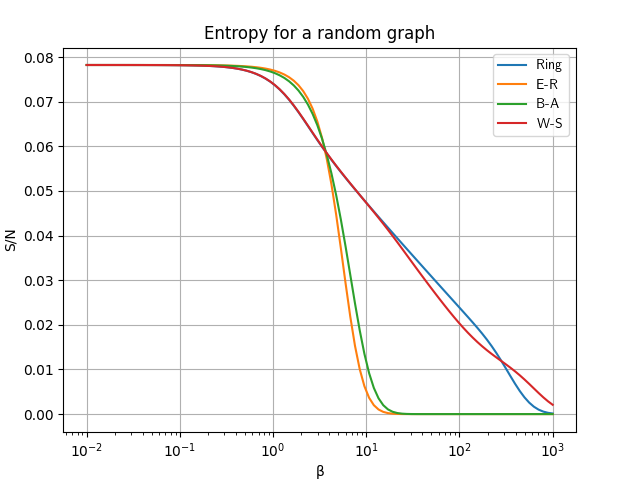
\includegraphics[width=0.75\linewidth]{image/random_graph.png}
    \caption{Plot of the network's entropy per node as a function of $\beta$ for different network types with $50$ nodes: a ring graph (blue), a Erd\H{o}s-Rényi (E-R) random graph with connectivity probability $0.7$ (orange), a Barab\'asi-Albert (B-A) scale-free graph with parameter $m=3$ (green), and a Watts-Strogatz (W-S) small world graph with parameter $K=3$ and rewire probability 0.2 (red). The x-axis has a logarithmic scale. For large $\beta$ the entropy tends to zero far all the networks.}
    \label{fig:ER-BA-WS}
\end{figure}

Using the density matrix, we can introduce also other thermodynamics quantities like the Helmoltz free energy $F = -\frac{1}{\beta} \ln Z$.


A possible interpretation of this density matrix is given by De Domenico \cite{De_Domenico_2020}.
Consider a network composed of $N$ nodes, encoded in the adjacency matrix $A$. Each node can be associated with a  value $n_i$ representing a property of the network, like the number of particles in the node in a diffusion model. 
The evolution of these variables is governed by the control operator $\hat L$. 

The network can be described using the Dirac notation. Let be $\ket{\psi} = \sum_i n_i \ket{i}$ the state of the system, where $\ket{i}$ is the canonical vector identifying the node $i$. The set $\{\ket{i}\}_{i=0}^N$ forms an orthogonal basis, satisfying $\braket{i}{j} = \delta_{ij}$, where $\delta_{ij}$ is the Kronecker delta.

The dynamics can be written as
\begin{equation} \label{time_evolution}
    \partial_t \ket{\psi(t)} = - \hat L \ket{\psi(t)},
\end{equation}
with the solution
\begin{equation}
    \ket{\psi(t)} = \hat G(t,0) \ket{\psi(0)}
\end{equation}
where $\hat G(t,0) = e^{-t\hat L}$ is the propagator and $\ket{\psi(0)}$ is the initial state. 

Since $\hat L$ is Hermitian, the propagator can be diagonalized in the orthogonal basis $\{\ket{v_\lambda}\}_\lambda$ of eigenvectors of the control operator
\begin{equation}\label{diagonal_propagator}
    \hat G(t,0) = \sum_\lambda e^{-t\lambda} \ket{v_\lambda}\bra{v_\lambda} = \sum_\lambda e^{-t\lambda} \hat \sigma_\lambda,
\end{equation}
where $\hat \sigma_\lambda$ is the projection over the left and right eigenvectors with the $\lambda$ eigenvalue. The operators do not depend on time, they are constant along the process, only the eigenvalues change.

The system relaxes to a stationary state $\ket{\psi_0}$ corresponding to the zero eigenvector.
We consider the system in the initial state $\ket{\psi} = \ket{\psi_0} + \ket{\Delta\psi}$, where $\ket{\Delta\psi}$ is a small perturbation relative to the stationary state. The initial perturbation can be decomposed as $\ket{\Delta\psi_0} = \sum_i \Delta_i \ket{i}$.
The time evolution of the state becomes
\begin{equation}
    \ket{\psi(t)} = G(t,0) \ket{\psi(0)} = \ket{\psi_0} + G(t,0)\ket{\Delta\psi} = \ket{\psi_0} + \ket{\Delta\psi(t)}
\end{equation}
with $\ket{\Delta\psi(t)} = e^{-t\hat L} \ket{\Delta \psi}$.

Since the stationary component is constant in time, we focus on the perturbation. 
The value of the perturbation at node $j$ at time $t$ is
\begin{equation}
    \braket{j}{\Delta\psi(t)} = \bra{j} e^{-t\hat L} \ket{\Delta\psi} =\sum_\lambda \bra{j} e^{-t\lambda} \hat \sigma_\lambda\ket{\Delta\psi} = \sum_i  \sum_\lambda \Delta_i e^{-t\lambda} \bra{j}  \hat \sigma_\lambda \ket{i}.
\end{equation}
We have used equation \eqref{diagonal_propagator} and the definition of the perturbation.
This equation shows that the perturbation travels through $N$ different streams, one for each $\sigma_\lambda$, with the stream's size $\Delta_i e^{-t\lambda}$. If $\Delta_i e^{-t\lambda} > 0$ the stream is active; if $\Delta_i e^{-t\lambda} = 0$ it is inactive. Negative stream coefficients imply an inverted flux from $j$ to $i$.
Sometimes, the dynamics traps part of the perturbation in a specific node. The trapped perturbation's size can be compute as
\begin{equation}
    T = \sum_i  \sum_\lambda \Delta_i e^{-t\lambda} \bra{i}  \hat \sigma_\lambda \ket{i} 
\end{equation} 

Assuming maximal uncertainty in the perturbation, obtainable when $\Delta_i = \Delta$, the equation reduces to
\begin{equation}
    T = \Delta \sum_i e^{-t\lambda} \bra{i}  \hat \sigma_\lambda \ket{i} = \Delta \Tr [\hat G(t,0)]
\end{equation}

Since the trapped perturbation regulates the stream's sizes, it can be responsible for the generation of the streams itself. 
Thus, we can define a density matrix 
\begin{equation}
    \hat \rho_t = \frac{1}{T} \Delta e^{-t\hat L} =  \frac{1}{Z} e^{-t\hat L},
\end{equation}
where $Z = \Tr[e^{-t\hat L}] $ is the partition function.
This density matrix can be interpreted as the probability that the perturbation will flow through a specific stream $\hat \sigma_l$ in the ensemble of all the possible streams \cite{De_Domenico_2020}.

The complexity of information streams can be quantified by the Von Neumann entropy.
When the information dynamics is described by a single information stream, a pure state, entropy is zero.
In contrast, as the information dynamics becomes more complex and diverse, the number of information streams increases, resulting in higher entropy.

\subsection{Kullback-Liebler and Jensen-Shannon Divergences}
Starting from the concept of entropy, we can also introduce the Kullback-Liebler (KL) divergence or relative entropy \cite{K-L_divergence} as
\begin{equation}\label{KL_divergence}
    D_{KL}(\hat \rho || \hat \sigma) = \Tr \left[\hat \rho \ln\left(\frac{\hat\sigma}{\hat\rho}\right)\right].
\end{equation}
It measure the close is the distribution $\hat \sigma$ to reproduce a event with real distribution $\hat \rho$. 
The KL divergence is always non negative and it equals zero when $\hat \rho = \hat \sigma$. It is not symmetric an unbounded \cite{J-S_divergence}.

It can be used to make comparisons between networks. Moreover, this concept we can be applied to the reconstruction of network starting from real data using the maximum likelihood estimation: it is to find the best model that reproduce the experimental data. In fact, the maximum likelihood estimation can be apply minimizing the Kullback-Liebler divergence between chosen network models and the dataset \cite{De_Domenico_2016}. This opens the door to the application of machine learning technique in complex network.


However the Kullback-Liebler divergence is not symmetric, therefore it can not be use as a metric. 
But we can symmetrize introducing the Jensen-Shannon (JS) divergence \cite{J-S_divergence} as
\begin{equation}\label{JS_metric}
    \mathcal{D}_{JS}(\hat\rho||\hat\sigma) =  \frac{1}{2}D(\hat \rho || \hat \mu) + \frac{1}{2}D(\hat \sigma || \hat \mu) = S(\hat\mu)-\frac{1}{2}\left[S(\hat\rho) + S(\hat\sigma)\right],
\end{equation}
where $\hat\mu =\frac{1}{2}(\hat\rho+\hat\sigma)$. 
\begin{figure}[ht!]
    \centering
    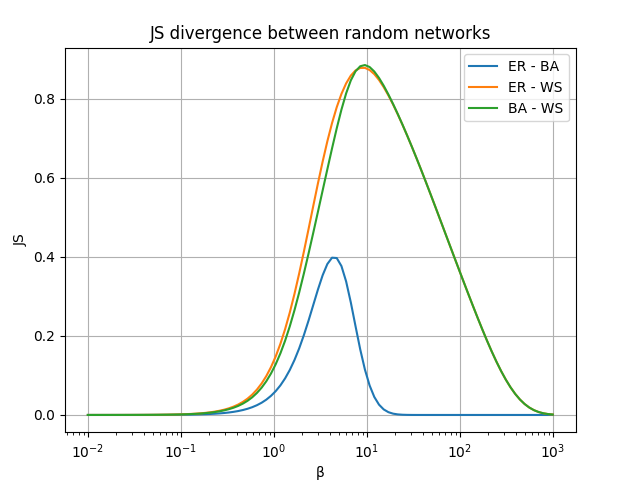
\includegraphics[width=0.75\textwidth]{image/JS_divergence.png}
    \caption{Plot of the KL divergence as a function of $\beta$ between different network types with $50$ nodes: a Erd\H{o}s-Rényi (E-R) random graph with connectivity probability $0.7$ and a Barab\'asi-Albert (B-A) scale-free graph with parameter $m=3$ (blue); a Erd\H{o}s-Rényi (E-R) random graph with connectivity probability $0.7$ and Watts-Strogatz (W-S) small world graph with parameter $K=3$ and rewire probability 0.2 (orange); a Barab\'asi-Albert (B-A) scale-free graph with parameter $m=3$ and a Watts-Strogatz (W-S) small world graph with parameter $K=3$ and rewire probability 0.2 (green). The x-axis has a logarithmic scale.The ER and BA networks are closer respect to a WS network. The divergence is maximum around $\beta = 10$.}
    \label{Fig:JS_divergence}
\end{figure}

The JS divergence is a bounded function \cite{J-S_divergence}
\begin{equation}
    0 \geq \mathcal{D}_{JS}(\hat\rho||\hat\sigma) \geq 1.
\end{equation}
$\left(\mathcal{D}_{JS}\right)^{\frac{1}{2}}$ defines a metric: it is symmetric, positive define, and hold the triangular inequality \cite{Jensen-Shannon_divergence}. 

%It has been use successfully to measure the distance between the layer of a multilayer network in order to aggregate them and eliminate the redundant layers \cite{multilayer}.
It has been use successfully to measure the distance between the network in order to aggregate them \cite{multilayer}.

Figure \ref{Fig:JS_divergence} shows the Jensen-Shannon divergence between an Erd\H{o}s-Rényi (E-R) random graph, a Barab\'asi-Albert (B-A) scale-free graph and a Watts-Strogatz (W-S) small-sworld graph \footnote{The python scripts can be found in the GitHub page of the author at the link: \url{https://github.com/ShqemzaMatteo/Master_thesis}}.